\documentclass[12pt]{article}
\usepackage{times}
\usepackage{tabularx}
\usepackage{fancyhdr}
\usepackage{float}
\usepackage{graphicx}
\usepackage[labelfont=bf]{caption}
\usepackage{subcaption}
\usepackage{natbib}
\usepackage{balance}
\usepackage{amsmath}
\usepackage{afterpage}
\usepackage[margin=1in]{geometry}
\usepackage{verbatimbox}

\def\title{High Level Hardware Construction in Chisel}
\def\author{Huy Vo}
\def\signatureA{Krste Asanovic}
\def\signatureB{Jonathan Bachrach}
\newcommand\blankpage{%
    \null
    \thispagestyle{empty}%
    \newpage}
%============ No need to modify anything below this line =================

%% \setlength{\leftmargin}{0.5in}
%% \setlength{\rightmargin}{0.5in}
%% \setlength{\topmargin}{0in}
%% \setlength{\textwidth}{6in}
%% \setlength{\textheight}{9.25in}
%% \setlength{\parindent}{0in}

\begin{document}

\section{Introduction}
\label{sec:intro}
Chisel~\cite{Bachrach:2012} is designed to be a {\it hardware construction language} so any
design in Chisel will always have a well defined mapping to low level
hardware blocks. Chisel's core programming features allow users to
accurately describe hardware circuits and can be easily extended for
higher level hardware designs. This paper categorizes Chisel hardware
construction into three levels and discusses the merits and drawbacks
of each level.

We first introduce the core features of the Chisel hardware
construction language in Chapter~\ref{sec:chisel}. All hardware design
in Chisel boils down to writing a Scala program that builds up a directed
graph of {\tt Nodes} which are Scala objects that map to basic circuit
elements. Chisel provides basic operators for constructing and
connecting nodes into subgraphs. The subgraphs can be organized into
{\tt Components} which can be connected to other {\tt Components} to
form larger and more complex graphs. Chisel code can be mapped to many
different backends. We currently support a C++ backend for high speed
simulation and a Verilog backend to leverage existing ASIC tools.

Chapter~\ref{sec:basic} presents the lowest level of hardware
construction in Chisel. We consider this the lowest level since
Chisel code is written at the granularity of Chisel's most basic
element, {\tt Nodes}. At this hardware construction level, Chisel user
code looks identical to the targeted backend code. This can be
advantageous if the backend has syntax that the tools can use to
synthesize efficient hardware. The downside to this is that syntax in
one backend might not have a parallel in another backend.

Moving up the abstraction ladder, Chapter~\ref{sec:advanced} presents
the next level of Chisel hardware construction in which the user
writes code using Scala functions that generate hardware. Although the
Chisel code might look similar to Chisel from Chapter~\ref{sec:basic},
the resulting Chisel graph is much denser since this hardware
construction level only uses the basic features of Chisel. Higher
level hardware facilities are abstracted away into Scala functions that
implement the same functionality using only basic Chisel {\tt
  Nodes}. Although we no longer leverage backend tool support for
special syntax, this approach has the advantage of decoupling Chisel
code from the backends.

The last level of hardware construction, Chapter~\ref{sec:elab},
analyzes and transforms Chisel graphs to produce different Chisel
graphs. This hardware construction level is similar to the hardware
construction level of Chapter~\ref{sec:advanced} in that users still
write Scala programs to build hardware. The difference is that these
functions are invoked during elaboration time to modify a graph
instead of during runtime to build the graph. This hardware
construction level is useful for circuit designs that are difficult or
undesirable to build during runtime.

\subsection{Related Works}
The most widely used hardware description languages (HDL), Verilog and VHDL,
are actually ill-suited for designing efficient, high-performance
hardware. These languages lack the powerful abstraction facilities
that are readily available in modern programming languages. Without
these facilities, hardware designers using these languages are
relegated to writing undescriptive and non-reusable hardware modules
which dramatically impedes the most important aspect of building
efficient hardware: design space exploration.

One way to circumvent this issue is to design hardware from within a
specific domain. Esterel~\cite{esterel} is synchronous programming
language that uses event-based statement to describe reactive
systems. Bluespec~\cite{bluespec} uses guarded atomic actions to
describe state change. Spiral~\cite{hoe:spiral} generates hardware
for linear signal transformations from an input problem
description. Although these languages allow designers to write more
expressive hardware, they only work well when used for task that
matches their model and will fall short when used for general purpose
hardware construction.

\subsection{Acknowledgments}
The Chisel HDL is an ongoing project. Jonathan Bachrach is the
original author. I joined the project in 2011 where I worked with
Jonathan and Brian Richards to port an existing FPU library from
Verilog to Chisel. I continued working with Jonathan to implement
Chisel's type system. In 2012 I work with Yunsup Lee to port an
existing vector machine to Chisel. During this time I developed Vec to
better express the hardware in the vector machine. I eventually moved
Vec into Chisel's library. Since then Jonathan has added support for
bidirectional wires to Vec and Andrew Waterman has added new
functionality to Vec such as {\tt contains} and {\tt forAll}
methods. Jonathan is responsible for the original implementation of
Chisel's {\tt when} statement. Andrew implemented Chisel's elaboration
time interface. Yunsup, Andrew, and I have written various SRAM
backends for the chips we built. The automatic pipeline synthesis tool
is CS294-88 class project that I developed with Wenyu Tang.

\clearpage
\section{Chisel}
\label{sec:chisel}
Chisel is a domain-specific language embedded in the Scala
programming language~\cite{scala} so it is really just a library of Scala functions
and data structures. Someone writing Chisel code is essentially writing a Scala
program that uses the provided functions and data structures to
construct hardware. This chapter introduces the core
components of the Chisel hardware construction language; readers
interested in a more a detailed specification of Chisel should consult
the Chisel manual~\cite{chisel:man} which can be found on the Chisel website. 

\subsection{Node}
Hardware circuits are represented in Chisel as directed graphs of
{\tt Nodes}, which are the base class from which all circuit elements are
derived. Figure~\ref{fig:hier} shows the Chisel class
hierarchy and Figure~\ref{fig:nodeapi} shows the API for the Node class.

{\bf Types}. Chisel has its own type system that is maintained
independent of the Scala type system. Figure~\ref{fig:hier} shows the
Chisel data types and their hierarchy (everything rooted at
{\tt Data}). {\tt Bits} is used to represent raw collection of bits,
{\tt Bool} is used to represent Boolean literals, and {\tt Num} is
used to represent numbers. Note that {\tt Num} has two subclasses,
{\tt Fix} and {\tt UFix} which are used for signed and unsigned
numbers respectively.

\begin{figure}[hb]
\centering
  \begin{subfigure}[t]{0.48\textwidth}
  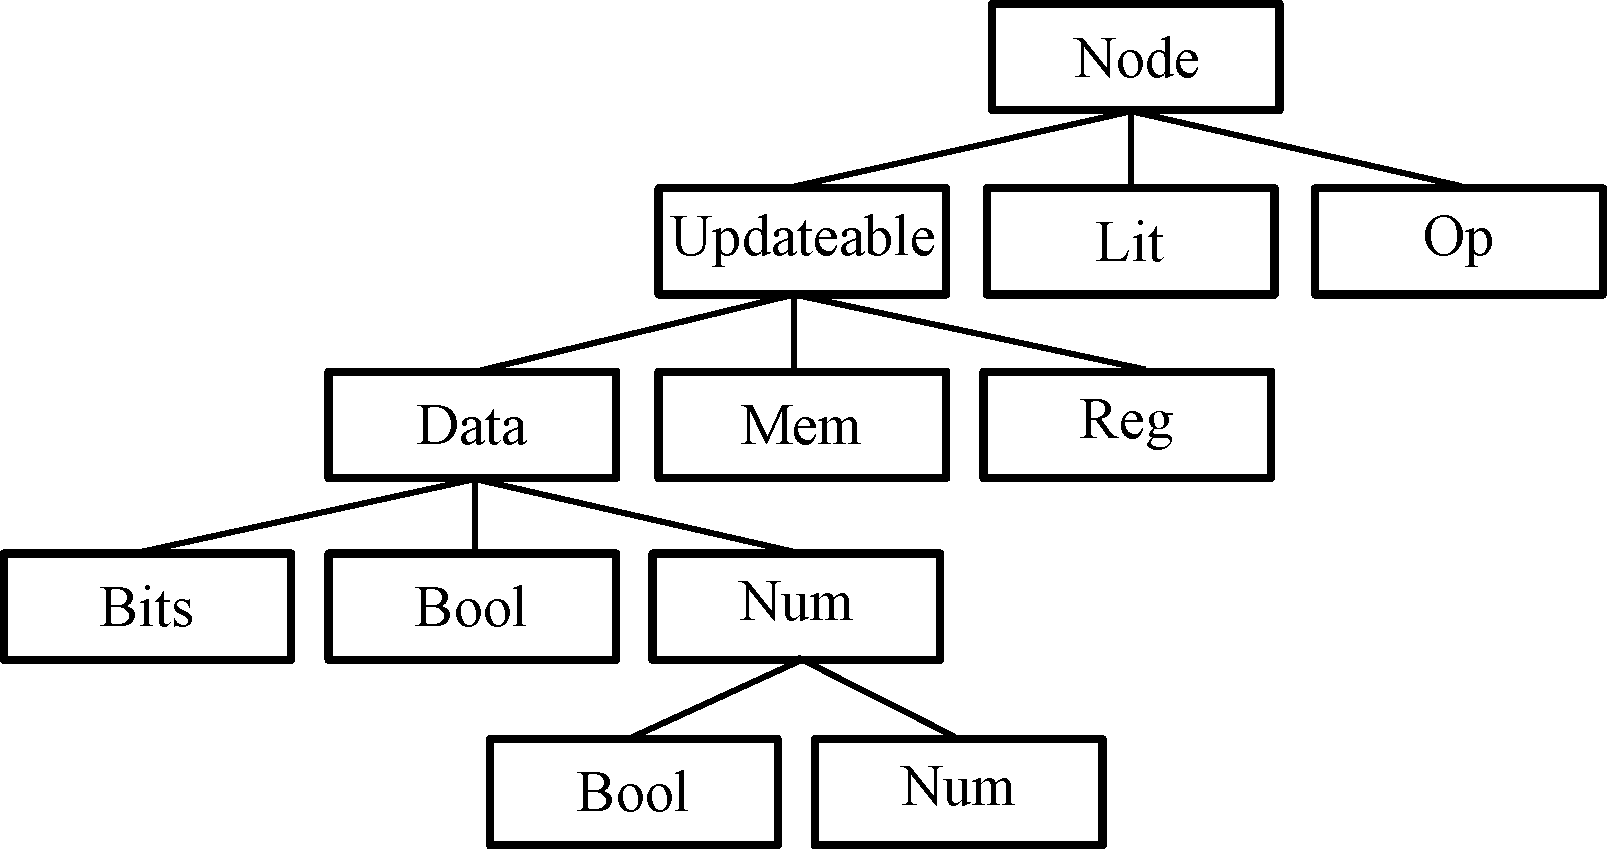
\includegraphics[width=\textwidth]{figures/hierarchy.pdf}
  \caption{Hierarchy}
  \label{fig:hier}
  \end{subfigure}
  \hfill
  \begin{subfigure}[t]{0.48\textwidth}
  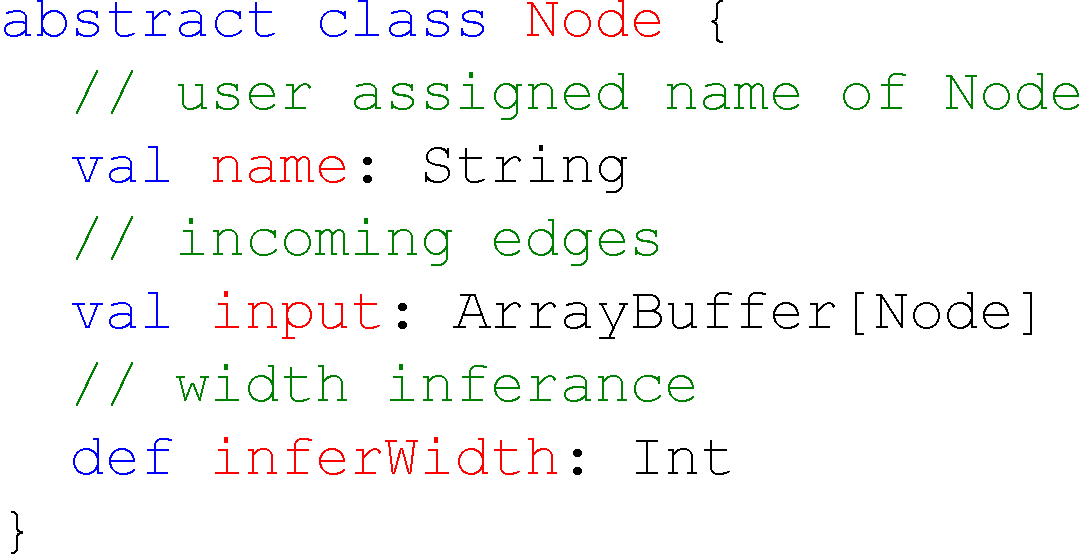
\includegraphics[width=\textwidth]{figures/node.pdf}
  \caption{API}
  \label{fig:nodeapi}
  \end{subfigure}
  \hfill
  \caption{Chisel Node}
  \label{fig:node}
\end{figure}

{\bf Arithmetic and Logic}. Arithmetic and logic operations
are represented with {\tt Op} nodes. The Chisel manual has an
exhaustive list of supported operations. Op nodes are constructed
whenever a user invokes the corresponding type node member
function for the operation. For example, suppose we have two {\tt
Bits} nodes, {\tt a} and {\tt b}, and want to connect them to the
inputs of an AND gate. The Chisel code that will do this is {\tt a \&
b} which is actually syntactic sugar for {\tt a.\&(b)}. The {\tt \&}
function that Bits defines will instantiate an {\tt Op} node to
represent the {\tt \&} and put the two {\tt Bits} nodes, {\tt a} and
{\tt b}, into the {\tt Op} node's input.

The example Chisel code in Figure~\ref{fig:mux} shows Bits nodes and
Op nodes interacting to create a 2-input multiplexor built out of {\tt
\&} and {\tt |} gates. In this example,  {\tt a}, {\tt b}, and {\tt
 sel} are incoming {\tt Bits}. Invoking {\tt a \& sel} will create a
new {\tt Op} and connect that node to a {\tt Bits} since both inputs
are {\tt Bits}. The output of the circuit, {\tt c}, will be the {\tt
Bits} connected to the {\tt |} {\tt Op}. 

\begin{figure}[t]
\centering
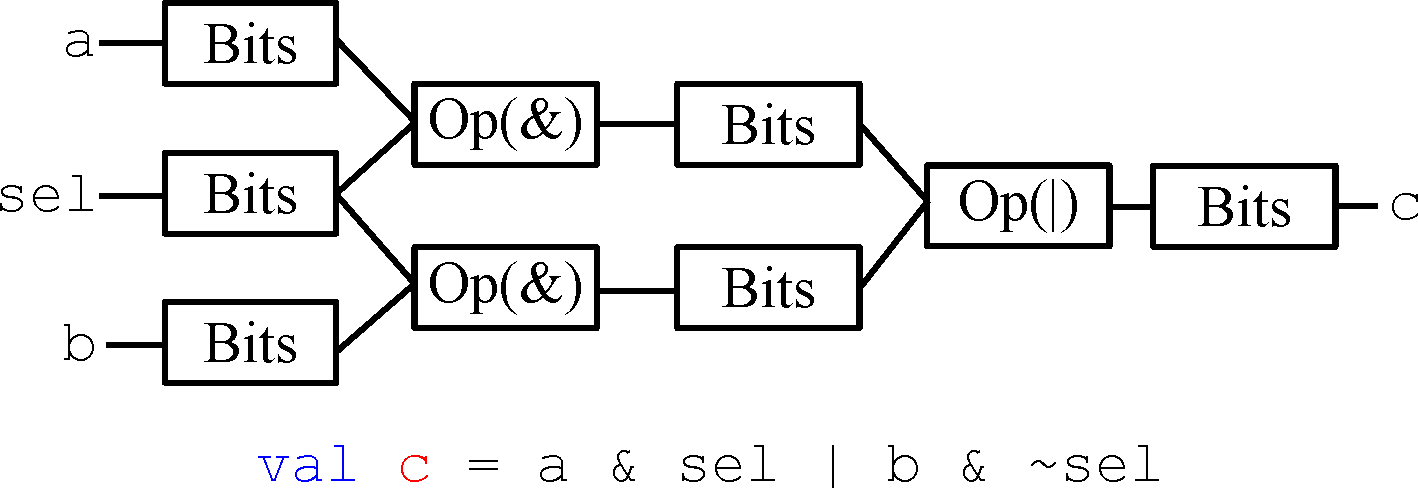
\includegraphics[width=0.75\textwidth]{figures/mux.pdf}
\caption{2-Input Mux}
\label{fig:mux}
\end{figure}

{\bf Literals} The {\tt Lit} node works in conjunction with type {\tt Nodes} to
represent literals. Figure~\ref{fig:lits} shows example Chisel code for
instantiating literals. True and false literals are represented as Bools
connected to {\tt Lit} nodes 1 and 0 respectively. Arbitrary bit
strings can be represented with {\tt Bits} Nodes and numbers can be represented with
{\tt Fix} and {\tt UFix} Nodes, all of which are connected to {\tt Lit
Nodes} with the appropriate value.

\begin{figure}[b]
\centering
  \begin{subfigure}[t]{0.22\textwidth}
  \centering
  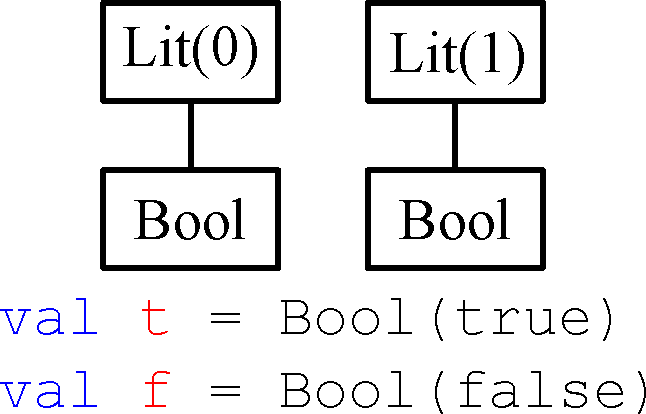
\includegraphics[width=\textwidth]{figures/bool.pdf}
  \caption{Bool literals}
  \label{fig:bool}
  \end{subfigure}
  \hfill
  \begin{subfigure}[t]{0.28\textwidth}
  \centering
  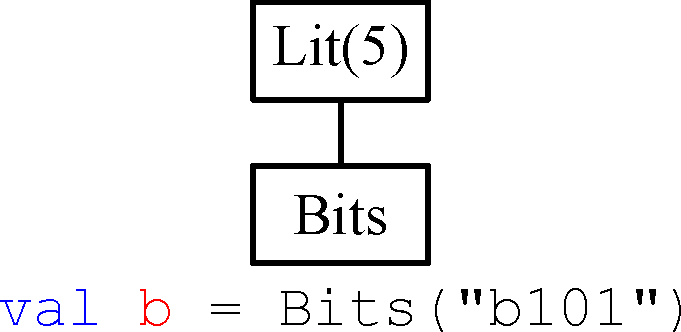
\includegraphics[width=\textwidth]{figures/bits.pdf}
  \caption{Bits literals}
  \label{fig:bits}
  \end{subfigure}
  \hfill
  \begin{subfigure}[t]{0.22\textwidth}
  \centering
  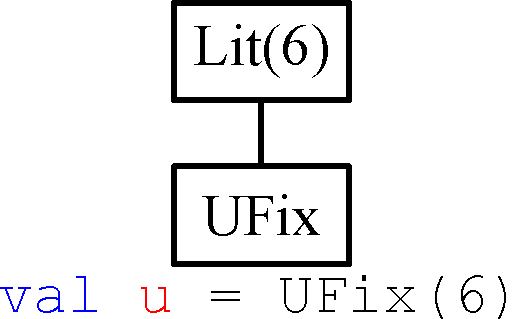
\includegraphics[width=\textwidth]{figures/ufix.pdf}
  \caption{UFix literals}
  \label{fig:ufix}
  \end{subfigure}
  \hfill
  \begin{subfigure}[t]{0.22\textwidth}
  \centering
  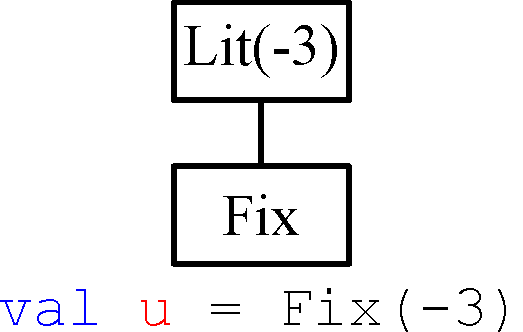
\includegraphics[width=\textwidth]{figures/fix.pdf}
  \caption{Fix literals}
  \label{fig:fix}
  \end{subfigure}
\caption{Chisel Literal Examples}
\label{fig:lits}
\end{figure}

{\bf Registers} The {\tt Reg} node, Chisel most basic state element,
represents a positive-edge-triggered flip-flop. {\tt Reg} nodes, unlike the
previous nodes, are manually instantiated by the user. The manual
details the different ways that a Reg can be constructed. Briefly,
Regs can be constructed either with or without an update signal.
{\tt Reg}'s constructed without an update signal can
be conditionally updated.

{\bf Memories} {\tt Mem Nodes} are used to represent random access
memories. These memories can be accessed with either {\tt Bits} or
{\tt UFix} nodes. Writes to these memories are positive-edge-triggered while
reads can be either combination or positive-edge-triggered.

\subsection{Component}
In addition to {\tt Nodes}, Chisel also provides {\tt Components} to allow users
to organize their directed graph of {\tt Nodes} into subgraphs, adding a
hierarchical structure to their hardware. Figure~\ref{fig:muxcomp} shows an
example of a Chisel implementation of a 4-input mux built from three 2-input muxes.

\begin{figure}
\centering
  \begin{subfigure}[t]{0.48\textwidth}
  \centering
  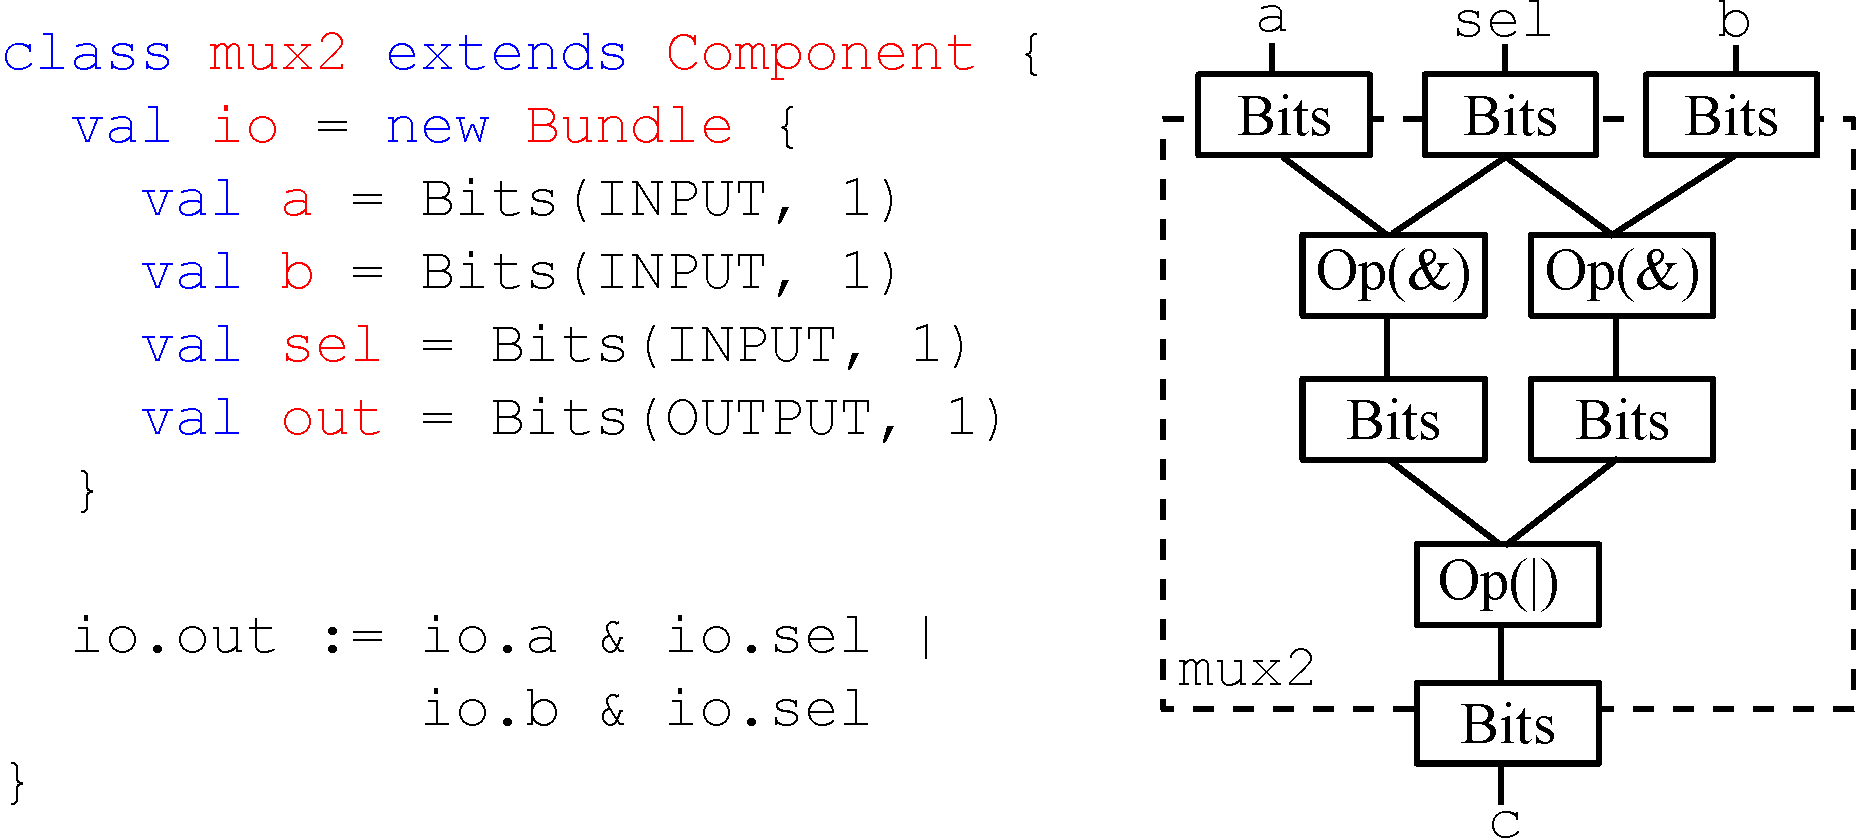
\includegraphics[width=\textwidth]{figures/mux2.pdf}
  \caption{2-Input Mux}
  \label{fig:mux2}
  \end{subfigure}
  \hfill
  \begin{subfigure}[t]{0.48\textwidth}
  \centering
  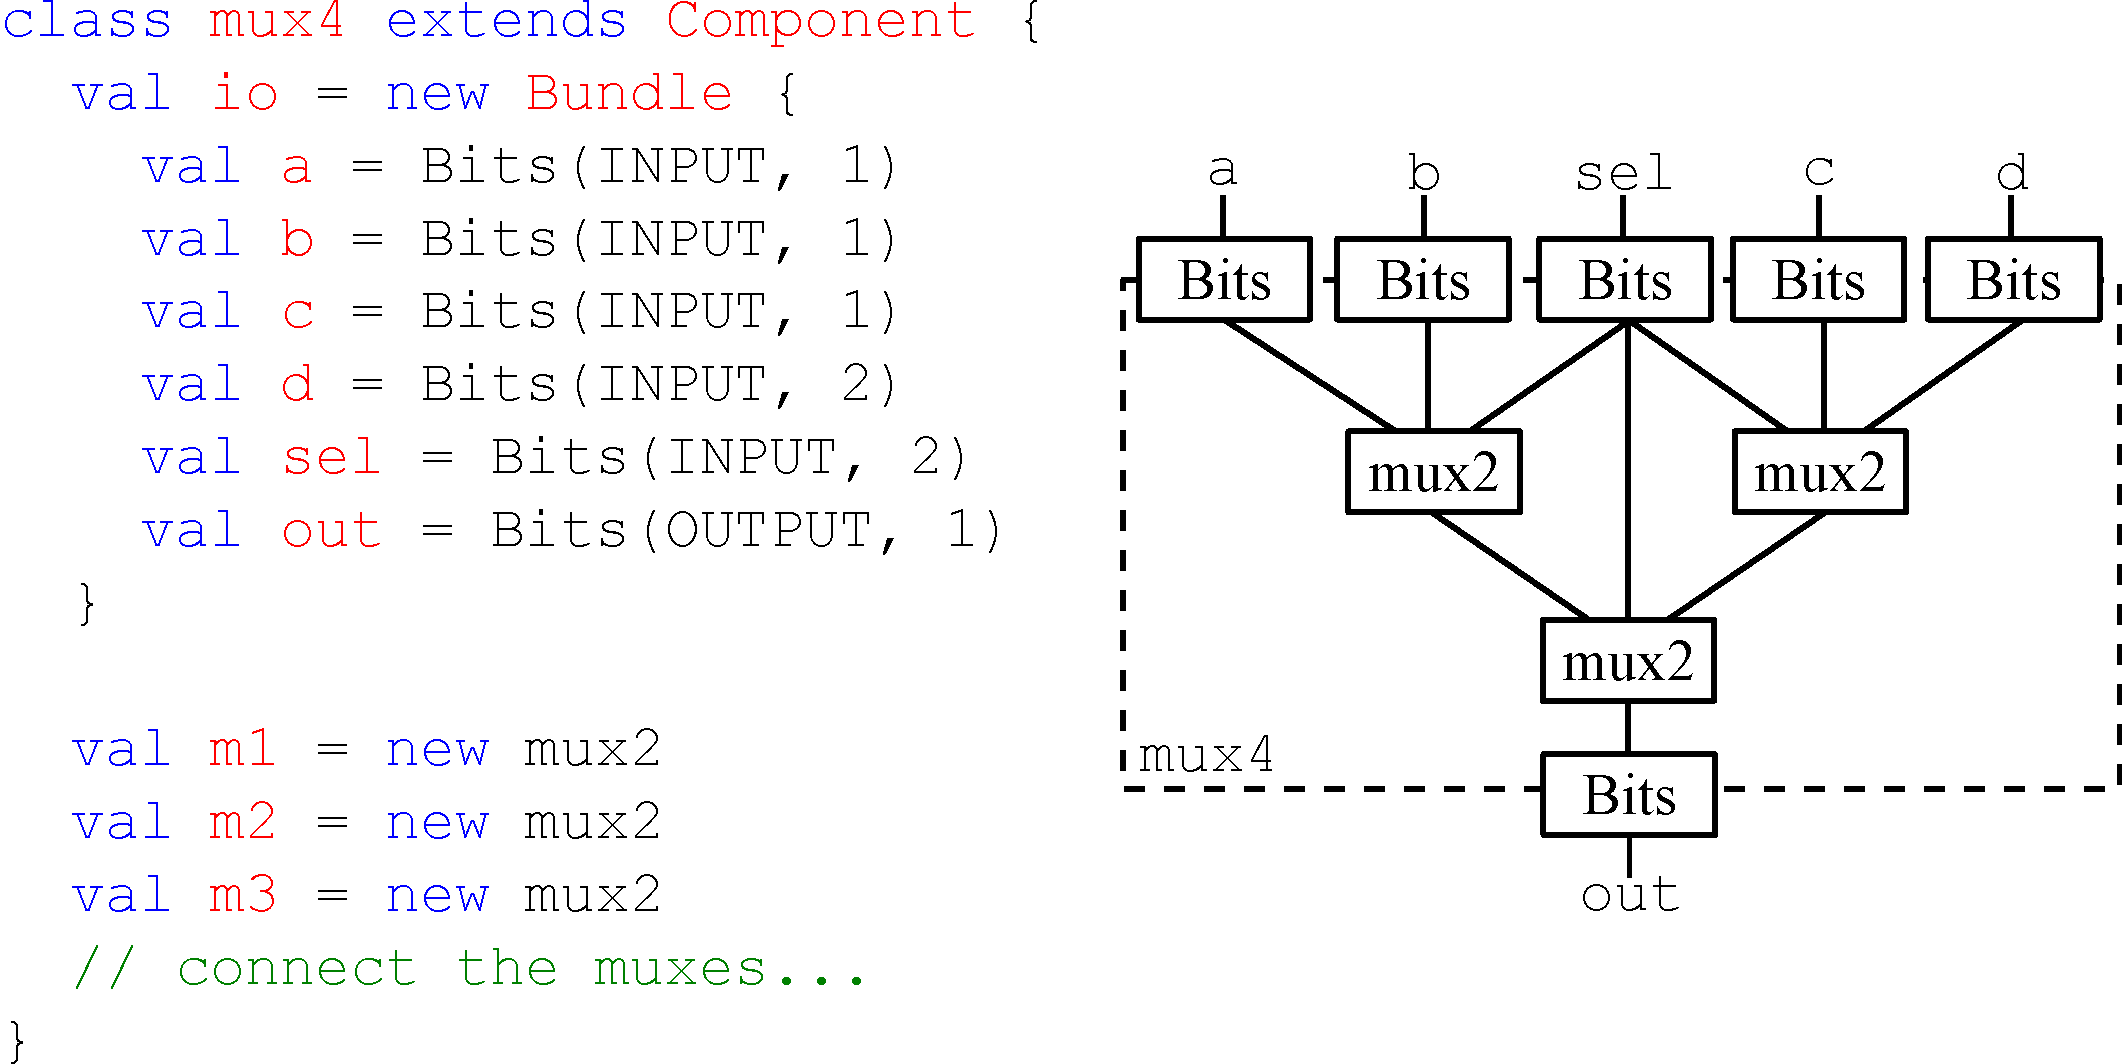
\includegraphics[width=\textwidth]{figures/mux4.pdf}
  \caption{4-Input Mux}
  \label{fig:mux4}
  \end{subfigure}
  \caption{Hierarchical 4-Input Mux}
  \label{fig:muxcomp}
\end{figure}

{\bf Interfaces} When defining a new Component, users have to fill out
the {\tt io} field which is the input-output interface that
Components expose to each other. An input or output node in Chisel is
represented with a type {\tt Node} where the direction field is set to
either {\tt INPUT} or {\tt OUTPUT}. The example in
Figure~\ref{fig:mux} shows Component interfaces built out of {\tt
Bits} nodes. Input and output nodes can be
collected into Bundles, which are functionally similar to C
structs, for better organization. 

{\bf Wiring} Once a Component's interface and circuit
implementation are defined, users will need to connect Components
together. Chisel provides two different ways for connecting
Components together. {\tt :=} is used for connections going from
right to left while {\tt <>} is used for connections that go in either
direction. Both connection operators can be used to connect either individual
ports or entire Bundles. If used for the latter, the connection
operator will recursively walk through Bundle and wire each element
individually.

\subsection{Backend}
The Backend takes as input a directed graph of {\tt Nodes} and
generates code for the specified backend. Figure~\ref{fig:backend}
shows how Chisel's backend generates code from a directed graph of
nodes. Chisel currently generates code for two backends: Verilog and C++.

{\bf Elaboration} The elaboration phase performs backend specific
transformation on the graph in order to generate valid code for that
backend. For example, it is desirable to preserve Component hierarchy
when targeting the Verilog backend, so the elaboration phase will do a
graph walk to match nodes into components. For the C++ backend, the
elaboration phase will transform the graph into a directed acyclic
graph and perform a topological sort.

The elaboration phase also performs transformations and checks that
are common to both backends such as width inference and combinational
loop detection.

\begin{figure}[!h]
\centering
  \begin{subfigure}[t]{0.48\textwidth}
  \centering
  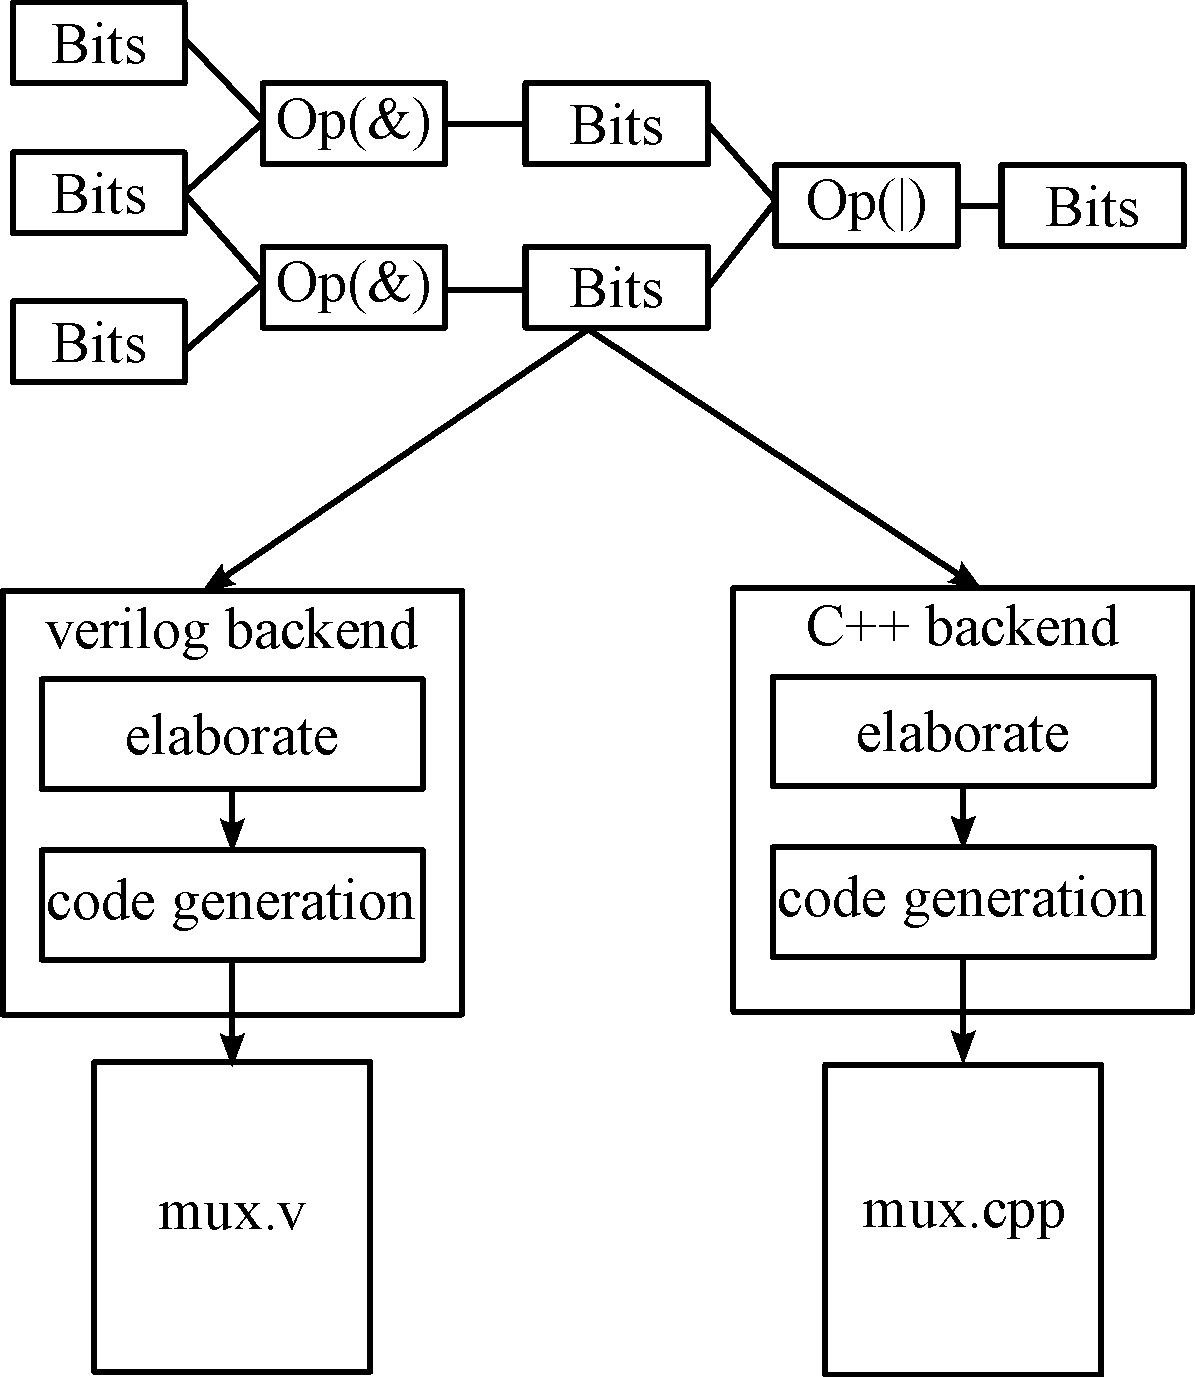
\includegraphics[width=0.7\textwidth]{figures/emit.pdf}
  \caption{Elaboration and Code Generation Process}
  \label{fig:emit}
  \end{subfigure}
  \hfill
  \begin{subfigure}[t]{0.48\textwidth}
  \centering
  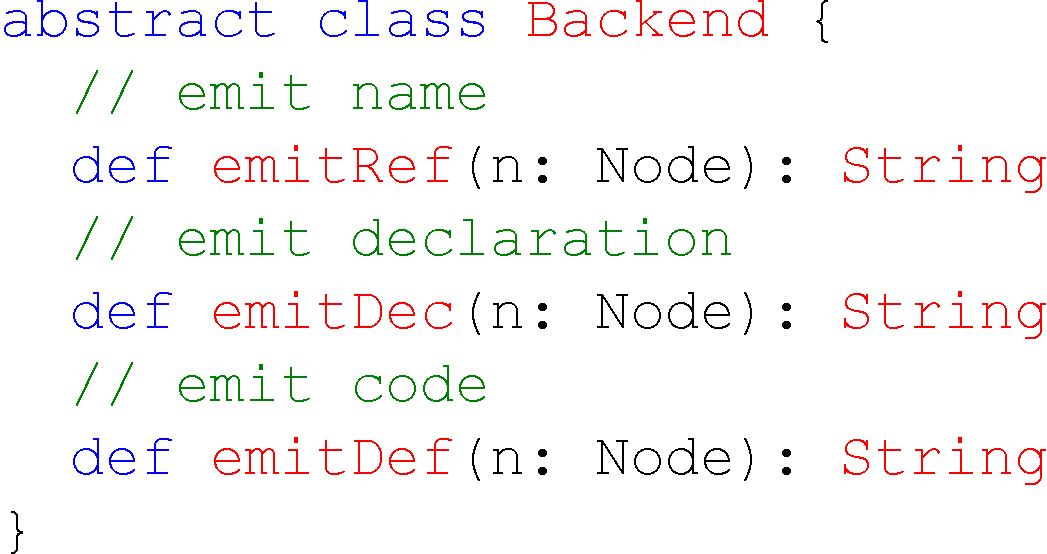
\includegraphics[width=\textwidth]{figures/backend.pdf}
  \caption{Backend API}
  \label{fig:backendapi}
  \end{subfigure}
\caption{Chisel Backend}
\label{fig:backend}
\end{figure}

{\bf Code Generation} Figure~\ref{fig:backendapi} shows the API for
generating code from an elaborated graph of nodes. The {\tt emitDec}
function is called to generate the code for declaring the node, {\tt
emitRef} is called to generate the reference to a node, and {\tt
emitDef} is called to generate the code. As an example, suppose the
Verilog backend is generating code for an {\tt Op} node that performs
an add. The {\tt emitDec} function, when called, returns the
string
\begin{align*}
\centering
\text{\tt{wire [31:0] a;}}
\end{align*}
assuming that the {\tt Op} is 32-bits wide and its user assigned name
is {\tt a}. The {\tt emitDef} function, when called, returns the
string
\begin{align*}
\centering
\text{\tt{assign a = b + c;}}
\end{align*}
assuming that the two nodes in the {\tt Op}'s input list have names
{\tt b} and {\tt c}.

\clearpage
\section{Basic Hardware Construction in Chisel}
\label{sec:basic}
The Chisel constructs presented in the previous chapter are adequate
for most hardware circuits. We have in fact built an entire floating
point library using only those constructs. Occasionally, users might
want to leverage syntax for hardware facilities available in a
target backend from within Chisel. Suppose for example that a user is
having Chisel target a backend that has support for highly optimized
FFT circuits. One way to leverage this facility is to introduce a new
type of {\tt Node} into Chisel that maps directly to that syntax in
the backend. This approach keeps the Chisel graph sparse since all the
hardware construction complexity is pushed into the backends where the
backend synthesis tools could possibly map the hardware facility to
very dense circuits. The downside to this approach is that Chisel code
using {\tt Nodes} designed to target these backend hardware facilities
now have a strong dependence on that backend. Furthermore, targeting a
new backend would require effort to port the Chisel user code if the
new backend does not have built-in support for the hardware facility.

The nuts and bolts to pay attention to when implementing a new 
{\tt Node} are the node's code generation functions and the node's
inputs list. Let's say we are implementing a new {\tt Node} called
{\tt Foo}. If {\tt Foo}'s code generation function need to reference
nodes {\tt B}, {\tt A}, and {\tt R}, then all three of those nodes
must go into {\tt Foo}'s input list. Omitting a node can lead to a
scenario where Chisel is unable to reach the omitted node and thus
never emits the backend code for that node. The result is 
{\tt Foo}'s backend code will make reference to non-existing hardware.
This chapter will show how {\tt ListLookup} and {\tt Vec} nodes can be
implemented to target Verilog's case statements and arrays.

\subsection{ListLookup}
\begin{figure}[htb]
\centering
  \begin{subfigure}[t]{0.48\textwidth}
  \centering
  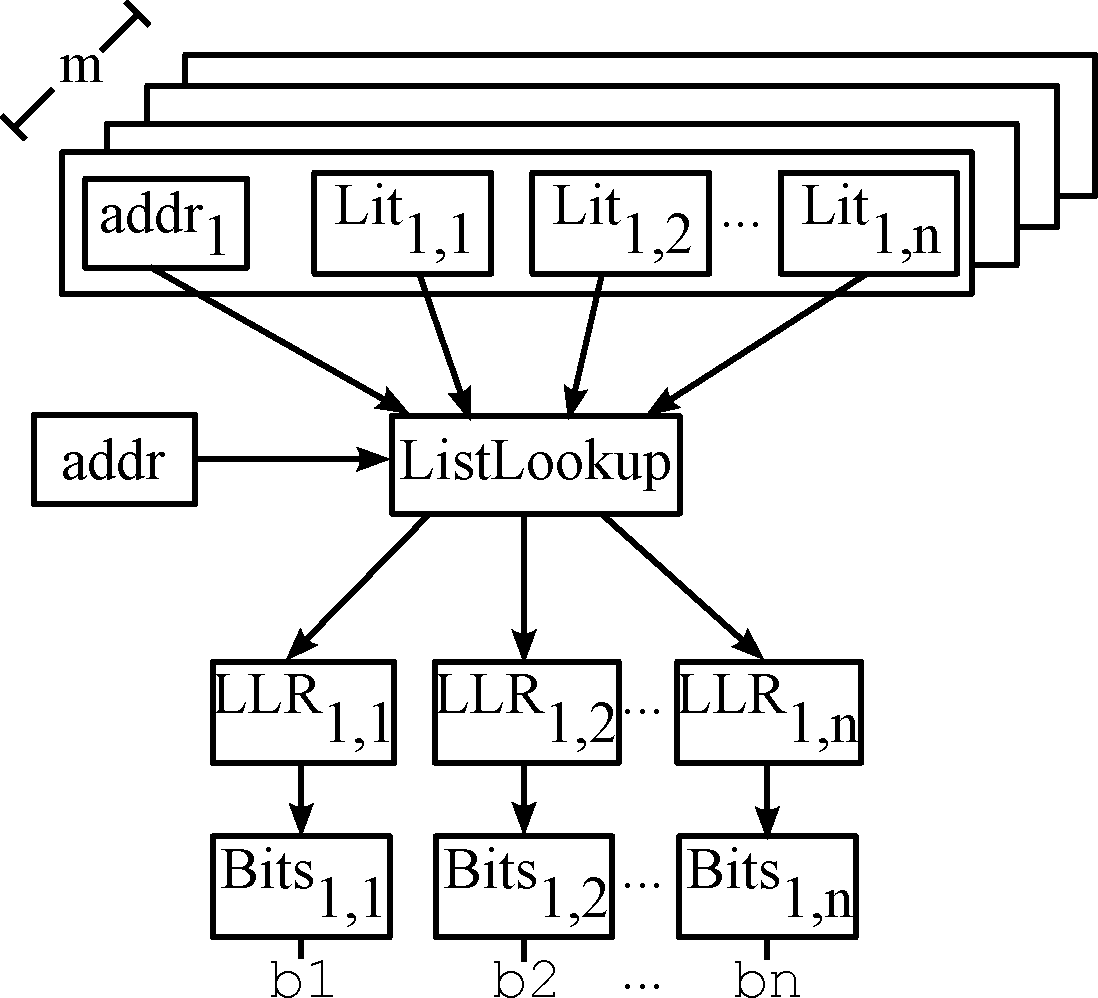
\includegraphics[width=\textwidth]{figures/listlookupnode.pdf}
  \caption{{\bf ListLookup Node}. Lit = {\tt Literal} node, LLR =
    {\tt ListLookupRef} nodes, and addr is shorthand for a {\tt Bits} node
    used as an address. Boxes with {\tt (addr$_j$,
      lits$_{i,j}$)} represent Scala tuples.}
  \label{fig:llnode}
  \end{subfigure}
  \hfill
  \begin{subfigure}[t]{0.48\textwidth}
  \centering
  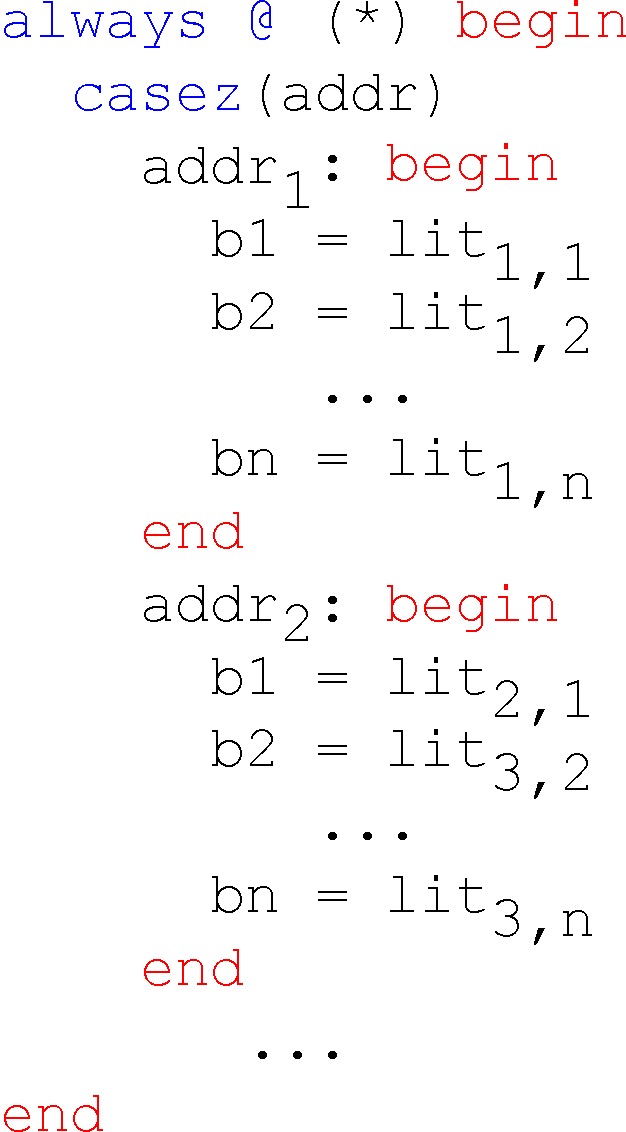
\includegraphics[width=0.5\textwidth]{figures/listlookupv.pdf}
  \caption{{\bf Generated ListLookup Code}. There are $m$ generated
    case statements each with $n$ literal assignments.}
  \label{fig:llv}
  \end{subfigure}
\caption{ListLookup as Chisel Node}
\label{fig:ll}
\end{figure}

\begin{verbbox}
ListLookup(addr: Bits, default: List[Lit], 
                       mapping: List[(addr, List[Lit])])
\end{verbbox}

We introduce {\tt ListLookup} and {\tt ListLookupRef} nodes to target
Verilog's case statement from within Chisel which is useful for
writing decode tables.

\textbf{ListLookup Node}.The inputs to this node are an address, a default list of literals,
and a list of tuples {\tt (a$_i$, lits$_i$)} where {\tt lits$_i$} is a list
of a literals. Figure~\ref{fig:llnode} shows how the inputs to the
{\tt ListLookup} nodes are managed. This node is different from other
nodes in that it does not have an entry for {\tt emitDec} and {\tt
emitRef}. The only code generation function it fills out is the {\tt
emitDef} function which generates the case statements in
Figure~\ref{fig:llv}. The ListLookup generates a case statement for
every {\tt (a$_i$, lits$_i$)} tuple where each case statements will
have an assignment for each literal in {\tt lits$_i$}. The address
input to the ListLookup is used as the lookup address into the case
statement and the {\tt a$_i$}'s are used to match against the
address. If no address matches, the default assignment is used.

\textbf{ListLookupRef Node}. Creating a new {\tt ListLookup} will not return
the {\tt ListLookup} to the user, rather, a list of 
{\tt ListLookupRef} nodes are returned instead. The length of the 
{\tt ListLookupRef} list matches the length of {\tt lits$_i$}. 
{\tt ListLookupRef} nodes do not have an entry for {\tt emitDef} since
the assignments to these nodes are actually done in the {\tt emitDef}
of a {\tt ListLookup} node.


\subsection{Vec}
\begin{figure}[hb]
\centering
  \begin{subfigure}[t]{0.48\textwidth}
  \centering
  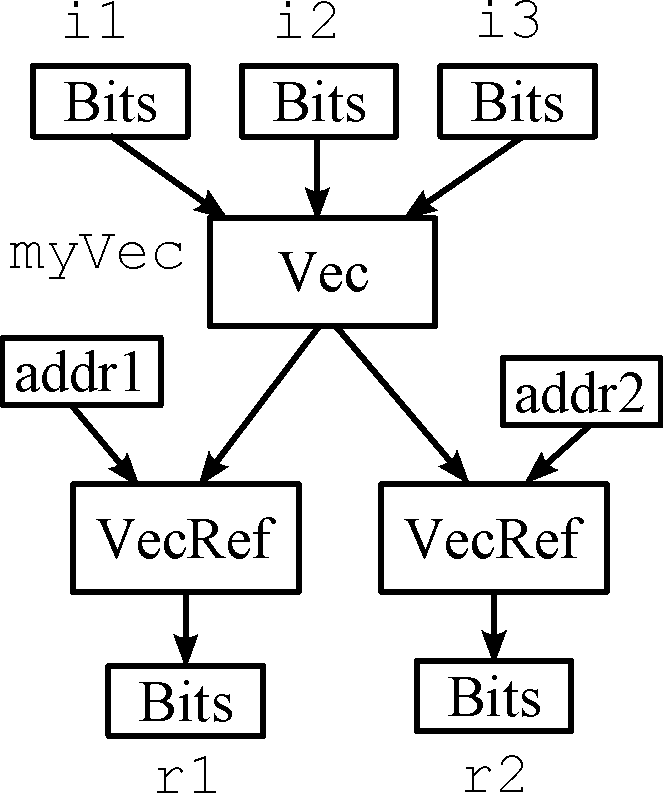
\includegraphics[width=0.5\textwidth]{figures/vecnode.pdf}
  \caption{{\bf Vec Node}. Example three entry {\tt Vec} with two
    read ports.}
  \label{fig:vecnode}
  \end{subfigure}
  \hfill
  \begin{subfigure}[t]{0.48\textwidth}
  \centering
  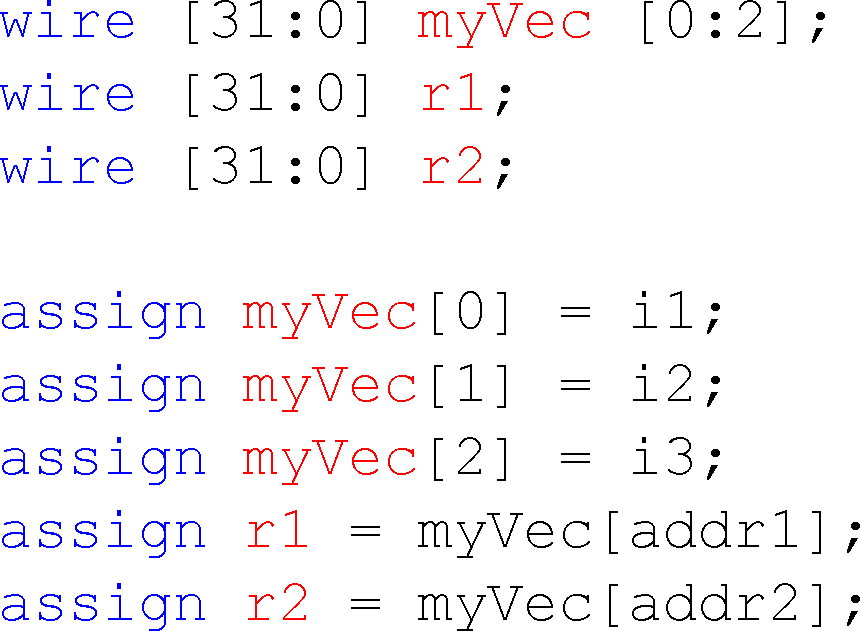
\includegraphics[width=0.7\textwidth]{figures/vecv.pdf}
  \caption{{\bf Generated Vec Code}. The two {\tt VecRef} nodes map to
  array accesses in Verilog.}
  \label{fig:vecv}
  \end{subfigure}
\caption{Vec as Chisel Node}
\label{fig:vec}
\end{figure}

We use {\tt Vec} and {\tt VecRef} nodes to target 2-D Verilog arrays
from within Chisel. Vecs are useful for organizing small collection of
wires into an indexable structure.

\textbf{Vec Node}. The {\tt Vec} node maps directly to the 2-D Verilog
array. Users instantiate this node with the desired number of entries
and then populate the node using {\tt :=}
assignments. Figure~\ref{fig:vecnode} shows a 3-entry {\tt Vec} where
the user has connected {\tt i1-3} to the {\tt Vec}. The width of a
{\tt Vec} node is inferred to be the maximum width of its inputs (in
this example, 32-bits wide). {\tt Vec}'s {\tt emitDec} function will
return the string
\begin{align*}
\centering
\text{\tt{wire [width-1:0] vec\_name [0:entries-1];}}
\end{align*}
where {\tt vec\_name} is the name of the node, {\tt width} is the
inferred width, and {\tt entries} is the number of entries in the
{\tt Vec}. The {\tt emitDef} function emits an assign statement for
each entry in the Vec.

\textbf{VecRef Node}. After instantiating and populating the Vec,
users will want to access the {\tt Vec} with dynamic addresses. Each
access with a new address will make a new {\tt VecRef} node. The
inputs to a {\tt VecRef} node are an address and a 
{\tt Vec} and its inferred with is the width of its input
{\tt Vec}. Figure~\ref{fig:vecnode} two {\tt VecRef} nodes made from
accessing the same {\tt Vec} with two different addresses. 
{\tt VecRef}'s {\tt emitDec} simply declares the name and width of the
node. Its {\tt emitDef} entry will return the string
\begin{align*}
\centering
\text{\tt{assign ref\_name = vec\_name[addr];}}
\end{align*}
where {\tt ref\_name} is the name of the {\tt VecRef} node, 
{\tt vec\_name} is the name of the {\tt Vec} and {\tt addr} is the
address.

\clearpage
\section{Advanced Hardware Construction in Chisel}
\label{sec:advanced}
Another way to support hardware facilities in Chisel, as opposed to
building new nodes, is to write a Scala program that aggregates the
features of Chisel from Chapter~\ref{sec:chisel} into a directed graph
of nodes that implement the same hardware functionality. This approach
moves the complexity of the hardware facility into the Scala graph but
makes the hardware facility much more accessible.
Unlike the approach from Chapter~\ref{sec:basic}, the
hardware facilities are now built out of basic Chisel {\tt Nodes} so
there is no dependence on backend support and no designer effort is
needed to target different backends. The downside is that the
resulting Chisel graph is much denser which would lenghten the time
spent in elaboration. We are also giving up on any optimization the
backend synthesis tool could provide for supported hardware facilities.

The hardware facilities built in this section will use the same syntax
as their counterparts from Chapter~\ref{sec:basic}. The difference now
is that we are reusing basic Chisel {\tt Nodes} and not implementing
new {\tt Nodes}. This chapter will show how to implement ListLookup
and Vec using only the basic Chisel nodes presented in
Chapter~\ref{sec:chisel}.

\subsection{ListLookup}
\begin{figure}[htb]
\centering
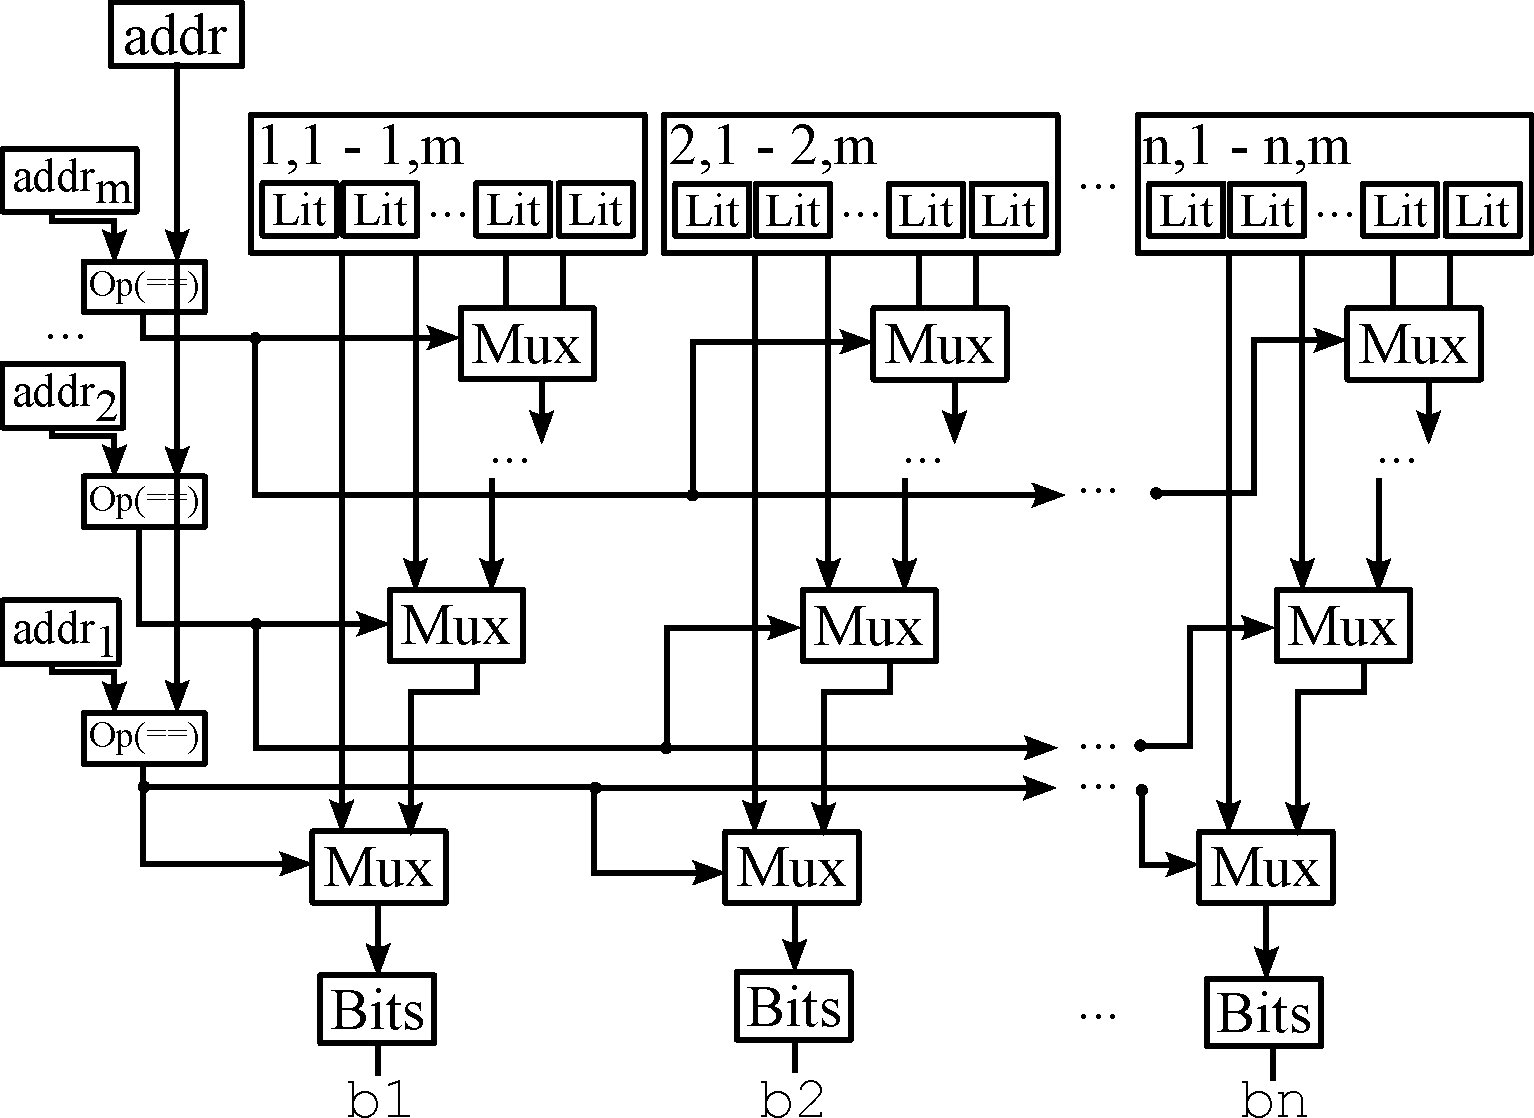
\includegraphics[width=0.7\textwidth]{figures/listlookupscala.pdf}
\caption{ListLookup implemented using Scala code and basic Chisel nodes}
\label{fig:llscala}
\end{figure}

The syntax for ListLookup remains the same. Users provide an address
for lookup and a list of size $m$ of tuples {\tt ($a_i$, $lits_i$)}
where {\tt $a_i$} is the address to match the lookup address against and
{\tt $lits_i$} is a list of size $n$ of literals to return when there
is a match. The ListLookup will then construct the graph in
Figure~\ref{fig:llscala}. The function returns a list of {\tt Bits}
{\tt $b_1$, ... $b_n$} who will take on the values of {\tt $lits_i$} if
{\tt $a_i$} matches the lookup address.

ListLookup graphs are constructed as follows. Given the input list of
tuples {\tt ($a_i$, $lits_i$)}, create $n$ list of $m$ tuples
{\tt $( (a_1, l_{1, k}), ... (a_j, l_{j, k}), ..., (a_m, l_{m, k})
  )$}. Each of these list represents a mux chain and there are $n$
such list ($k$ ranges from 1 to $n$). The mux chains are constructed
using {\tt $a_i$ === addr} as the select signal to the corresponding
mux. If the address matches, then literal {\tt $l_{i, k}$} is outputted
for Bits $b_k$.

\subsection{Vec}
\begin{figure}[htb]
\centering
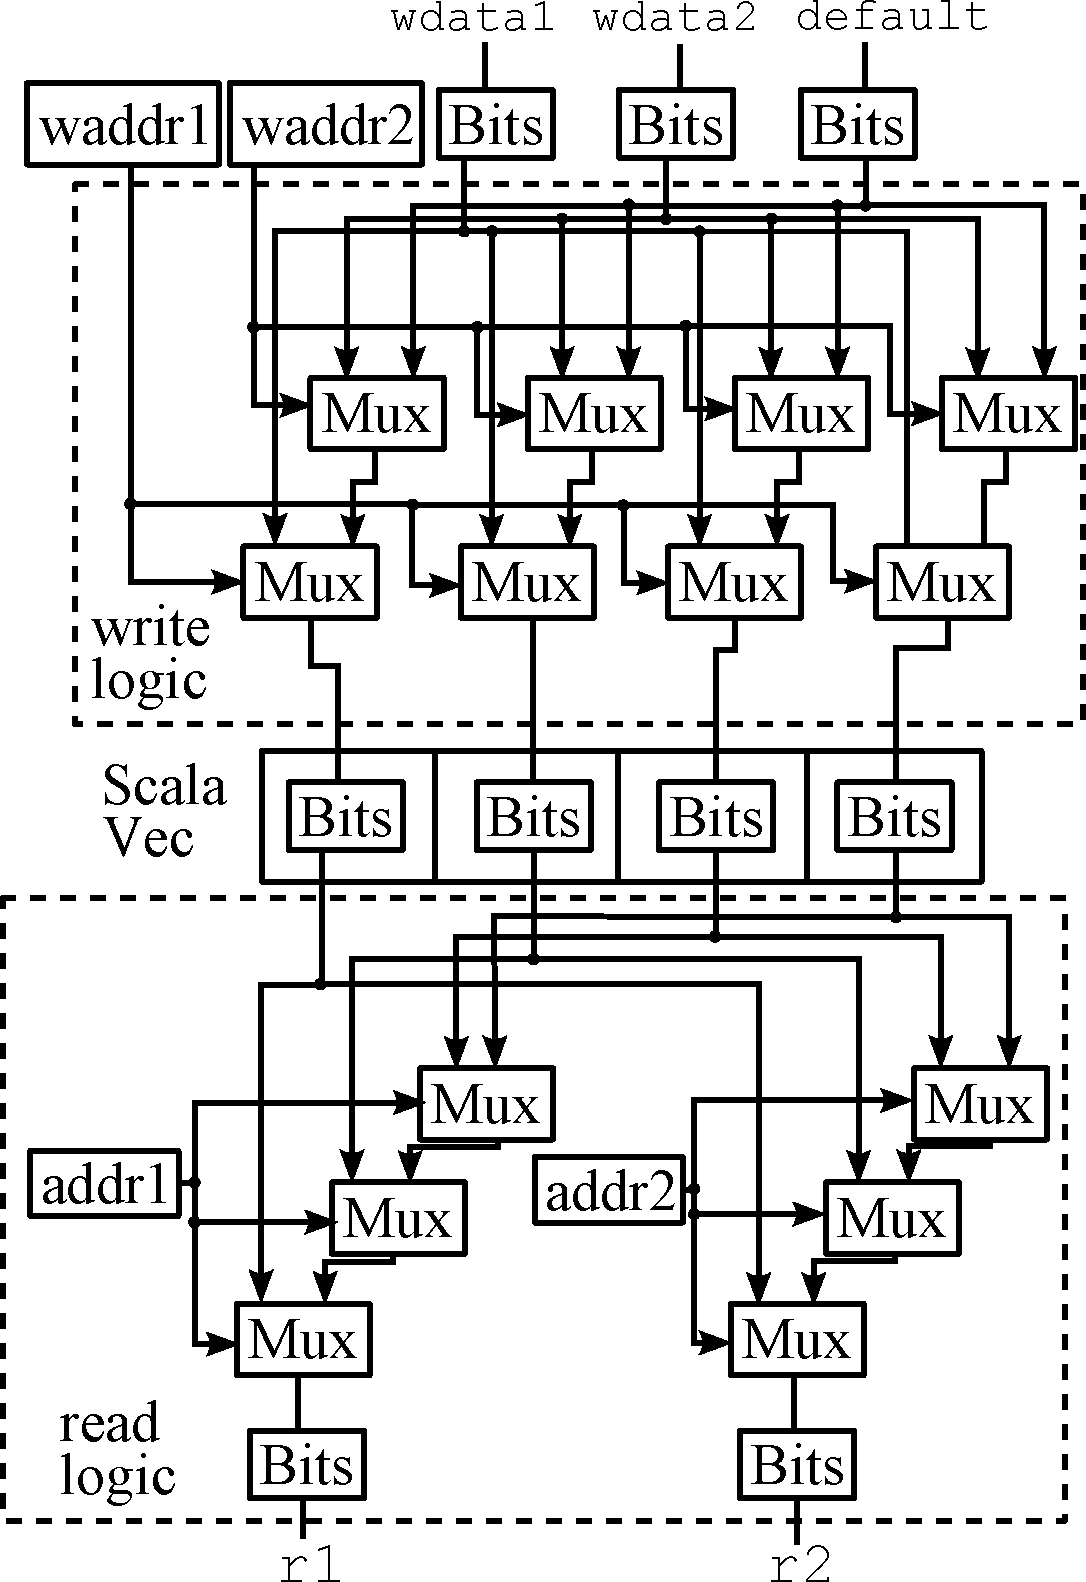
\includegraphics[width=0.5\textwidth]{figures/vecscala.pdf}
\caption{Vec implemented using Scala code and basic Chisel nodes}
\label{fig:vecscala}
\end{figure}

Figure~\ref{fig:vecscala} shows the resulting graph from building a
Vec using only basic Chisel nodes. Note that Vec is now a Scala array
of {\tt Bits} and is not a {\tt Node}. The syntax for constructing a
Vec is unchanged; users instantiate the Vec with the desired
size. Since the Vec is now a Scala array, users populate the Vec using
Scala array syntax, e.g.
\begin{align*}
  \text{ \tt{v(1) = Bits(width=32)} }
\end{align*}
where {\tt v} is the name of the Vec. The syntax for reading and
writing to the Vec is also unchanged. The difference is that reads
and writes will now construct the graph in Figure~\ref{fig:vecscala}
instead of instantiating special read and write nodes.

\textbf{Reads} A Vec can be indexed with either Scala integer or a
Chisel {\tt Node}. If a Scala integer is used, no {\tt Nodes} are
created and the element at that index is returned. If a Chisel 
{\tt Node} is used, then a Mux chain is built to mux out the correct
element of the Vec. The select signal to the mux is {\tt addr === idx}
where {\tt addr} is the address and {\tt idx} ranges from zero to
length of the Vec minus 1. When {\tt addr} matches an {\tt idx}, the
element at {\tt v(idx)} is outputted.

\textbf{Writes} Like reads, a Vec can be written to using either a
Scala integer or a Chisel {\tt Node} for indexing. If a Scala integer
is used, then the corresponding element is accessed and written to and
no nodes are constructed. If a Chisel {\tt Node} is used, then a mux
is placed in front of each element in the Vec. The select signal to
the mux is {\tt waddr ==== idx} where {\tt waddr} is the input write
address and {\tt idx} ranges from zero to the length of the Vec minus
1. If the write address matches the {\tt idx}, then the element at
{\tt v(idx)} is written to with the write data, otherwise {\tt v(idx)}
is written to with the default data. If the {\tt Vec} contains 
{\tt Bits} then the user supplies the default data. If the {tt Vec}
contains {\tt Reg} nodes then no default signal is needed.

\clearpage
\section{Elaboration Time Hardware Construction}
The methods for constructing hardware in the previous chapters are all
similar in that the user directly interfaces with them. The user
directly constructs the directed subgraph of {\tt Nodes} that
implements the desired circuit and connects that subgraph to the main
graph. We refer to that class of hardware construction as 
{\it runtime} hardware construction since the hardware is
constructed as Scala is making a pass over user-written code. This
chapter discusses another class of hardware construction that we refer
to as {\it elaboration time} hardware construction since the
hardware is constructed during Chisel elaboration. This class of
hardware construction is useful since it is not always possible or
desirable for the user to construct the circuit as they are building
up the Chisel graph. The remainder of this chapter presents the
interface for writing elaboration time hardware construction routines
and three examples of how to use that interface.

\subsection{Elaboration Time Hardware Construction Interface}
The Chisel compiler maintains a list of functions that it invokes
during elaboration time to refine the input user graph of 
{\tt Nodes}. These functions must adhere to the interface described in
Figure~\ref{fig:transforms}. The bodies of the functions in
Figure~\ref{fig:transform1} varies from transformation to
transformation but will usually follow two phase format. The first
phase performs some analysis on the Chisel graph to collect
information, e.g. find all Reg nodes. The second phase will then use
the information from the first phase to construct a circuit and
perform some transformation on the graph, e.g. generate an enable
circuit for every Reg node and connect the circuit into the Reg node.

\begin{figure}[htb]
\centering
  \begin{subfigure}[t]{0.48\textwidth}
  \centering
  \caption{Elaboration Time Functions}
  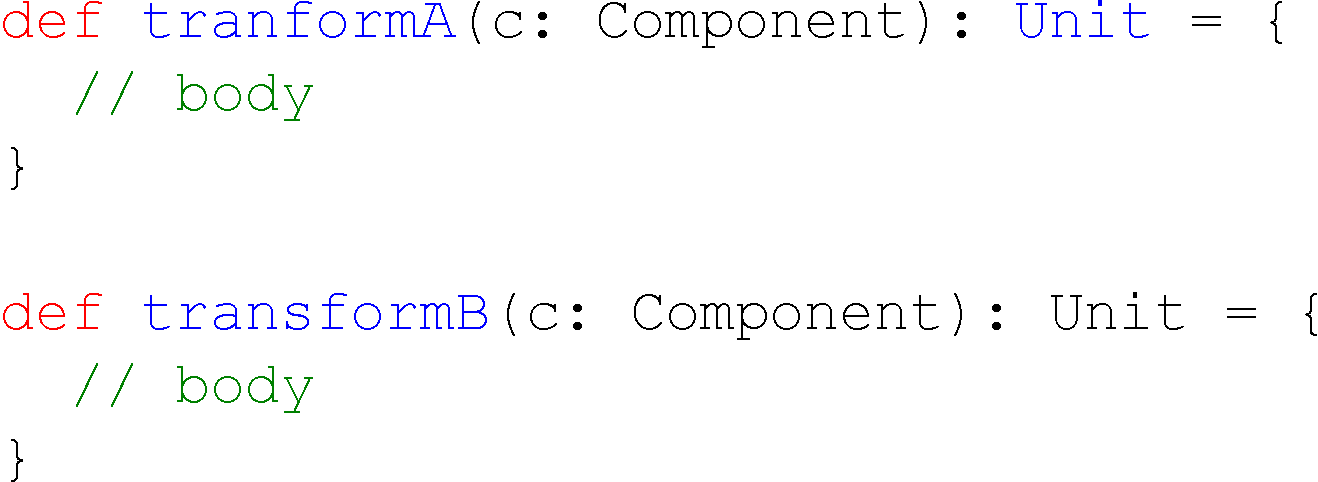
\includegraphics[width=0.9\textwidth]{figures/transform1.pdf}
  \label{fig:transform1}
  \end{subfigure}
  \hfill
  \begin{subfigure}[t]{0.48\textwidth}
  \centering
  \caption{Elaboration Time Hook}
  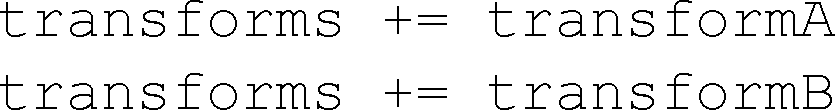
\includegraphics[width=0.7\textwidth]{figures/transform2.pdf}
  \label{fig:transform2}
  \end{subfigure}
\caption{Elaboration Time Interface}
\label{fig:transforms}
\end{figure}

\subsection{When}
Chisel provides a {\tt when - elsewhen - otherwise} statement for
performing conditional updates on {\tt Bits} and {\tt Reg}
nodes. This statement appears behavioral but actually constructs a
hardware circuit to perform the update. The construction of this
circuit is delayed until elaboration time since it is easier to
construct the circuit once the user has specified all the updates than
it is to construct the circuit as the user is specifying
updates. 

\begin{figure}[htb]
\centering
  \begin{subfigure}[t]{0.48\textwidth}
  \centering
  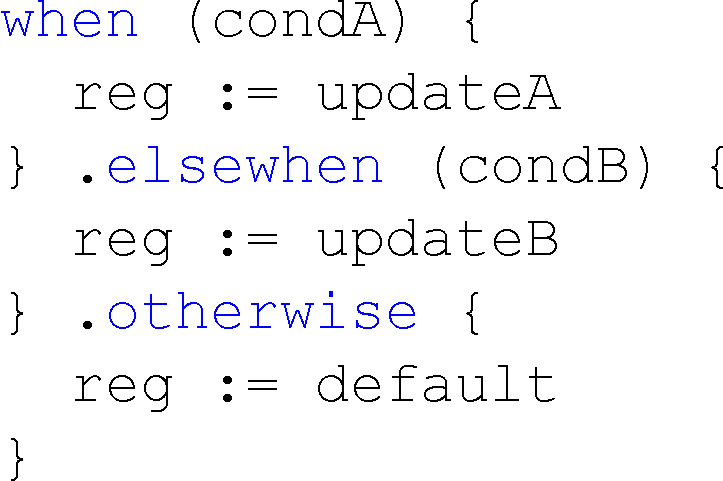
\includegraphics[width=0.7\textwidth]{figures/when.pdf}
  \caption{When Code}
  \label{fig:whenscala}
  \end{subfigure}
  \hfill
  \begin{subfigure}[t]{0.48\textwidth}
  \centering
  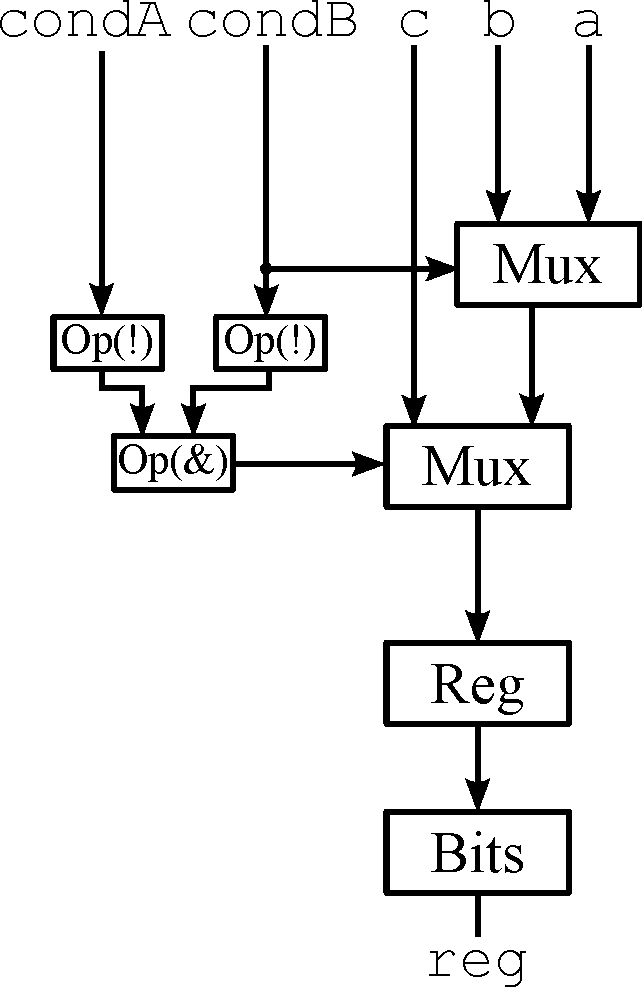
\includegraphics[width=0.5\textwidth]{figures/whengraph.pdf}
  \caption{When Graph}
  \label{fig:whenelab}
  \end{subfigure}
\caption{When Statement}
\label{fig:when}
\end{figure}

{\bf Runtime}. Instead of constructing hardware whenever a {\tt when}
statement is executed, we simply record information to be used during
elaboration. For this purpose, we maintain a mapping of node to list
of update tuples with the format {\tt (cond, bits)} where {\tt cond}
is the condition of the when statement and {\tt bits} is the update
data. These update tuples are constructed for every update statement
within the body of a {\tt when} statement and appended to the list
mapped to the node on the left hand side of that update
statement. Note that the updates in this list do not have to be
mutually exclusive. In the case when multiple updates are enabled,
Chisel has the semantics that the last update in program order (i.e
the last update in the list of updates) takes priority.

Figure~\ref{fig:whenscala} shows an example usage of when statements
to conditionally update a register. When this statement is executed,
it will add 3 update tuples to {\tt reg}'s list of update tuples. The
first statement adds the tuple {\tt (condA, updateA)}, the second adds
{\tt (condB \&\& !condA, updateB)}, and the third adds
{\tt (!condB \&\& !condA, updateC)}.

{\bf Elaboration Time}. The elaboration time transformation function
does not need to perform any analysis since we store all the
information for elaboration during runtime in the form of a mapping
from node to list of update tuples. For each entry in this mapping, we
construct a chain of {\tt Mux} nodes from the list of update tuples and
connect the output of that chain into the input of the node in the
mapping. If the node in the mapping is a {\tt Reg} node then nothing
is done for the case when no updates are enabled. Otherwise, the node
in the mapping is a {\tt Bits} node and we have an additional {\tt Mux}
node to mux out a default signal provided by the user. If no default
signal is provided, Chisel reports an error to the user.

\subsection{SRAM Backend}
Users targeting the Verilog backend will want to map Mems to SRAMs
with backend specific SRAM interfaces. One way to target these SRAM
interfaces is to encode the interface into the Chisel user code. This
has the disadvantageous effect of muddling the code with SRAM specific
information and makes it an unnecessarily tedious to compile the Chisel
for a different SRAM backend.

A better way to target backend specific SRAM interfaces is to write an
elaboration time function that transforms the Chisel graph to target
specific SRAM interfaces. Let's say we want to target an SRAM that has
an {\tt init} pin which needs to be wired to the top level module. We
first perform either a breadth first search or depth first search to
find all {\tt Mem} nodes in the graph. For every {\tt Mem} node, we
create a new {\tt Bits} node to stand in for the {\tt init} pin. We
add this node to the {\tt Mem} node's input. Finally, we walk up the
{\tt Component} hierarchy starting at the {\tt Component} that
contains the {\tt Mem} node and ending at the top level
{\tt Component}. For every {\tt Component} along this path, we create
a new port to connect up the {\tt init} pin.

Targeting SRAM interfaces in this way allows us to decouple of the
SRAM backend from the user code. If we want to switch to a different
SRAM target we only need to switch to a different elaboration time
function and do not need to modify the user code.

\subsection{Automatic Pipeline Synthesis}
Pipelining is a commonly used microarchitectural technique for
improving the performance of a datapath. Hardware designers usually
determine upfront the desired pipeline depth and then bake the
corresponding pipelining logic into their datapath code. This approach
clutters an otherwise easily readable datapath with extraneous logic
unrelated to original functionality of the datapath, making it
difficult to modify the datapath or even change the pipeline depth. A
better approach that overcomes these issues is to move the pipelining
logic into elaboration time functions.

{\bf Pipeline Specification}. In a hand coded pipeline, the pipeline
depth and the placement of pipeline registers are baked into the
Chisel datapath code. Our approach provides the functions 
{\tt setNumStages} for specifying the pipeline depth, 
{\tt setPipelineComponent} for specifying the datapath to pipeline,
and {\tt addToPipeline } for specifying in what pipeline stage a {\tt Node}
or {\tt Component} belongs. These functions allow the user to
succinctly describe a pipeline and unclutters the datapath code since
these functions can be maintained independent of the datapath.

{\bf Pipeline Generation}. The pipeline specification functions record
information that is read during elaboration time to add pipeline
registers to the directed graph of {\tt Nodes} that the Chisel datapath
code constructs.

{\bf Hazard Detection}. Inserting pipeline registers into the datapath
graph introduces pipelining hazards that are not present in the
unpipelined datapath. Here we discuss how to handle data hazards which
result from a transaction reading a state element (a {\tt Reg} node or
{\tt Mem} node) before an earlier transaction writes to that state
element. 

We first search through the datapath graph to find all state
elements. For every state element, we determine whether or not a
hazard exists on it. If there is a hazard on a state element, we add
the hazard condition into a list. For {\tt Reg} or {\tt Mem} node, a
hazard condition exists if the node belongs in a stage that precedes the
stage of its write enable or write data signal. The actual Boolean
hazard condition is {\tt wen \&\& ren} for a {\tt Reg} node and
{\tt wen \&\& ren \&\& waddr == raddr} for a {\tt Mem} node.

{\bf Hazard Resolution - Interlocks}. The easiest way to resolve
hazards is through interlocks. This hazard resolution method requires
no additional input from the user. At the stage of every state element
with a hazard condition, we trigger a stall at that stage and all
preceding stages while inserting a bubble in the following stage until
the hazard condition is no longer asserted.

{\bf Hazard Resolution - Speculation}. Some hazards can be resolved
through speculation. In a processor pipeline, for example, we can use
speculation to remove interlocks on the PC register. Users identify
speculation points.

{\bf Hazard Resolution - Bypassing}. Bypass networks can be built to
forward results from later stages to earlier stages that need the
result instead of forcing the earlier stages to stall until results
are committed. Users identify bypassing points.

\clearpage
\bibliographystyle{abbrvnat}
\setlength{\bibsep}{0.0pt}
\renewcommand*{\bibfont}{\footnotesize}
\bibliography{references}

\end{document}
